\documentclass[10pt,a4paper]{article}
\usepackage[utf8]{inputenc}
\usepackage[german]{babel}
\usepackage[T1]{fontenc}
\usepackage{amsmath}
\usepackage{amsfonts}
\usepackage{amssymb}
\usepackage{graphicx}
\usepackage{lmodern}
\usepackage{bm}

\author{Lars Schiller}
\begin{document}


\section{Problem Statement}

\begin{itemize}


\item Angenommen die Konfiguration / Pose des Roboters $\bm{\rho} = [\bm{\alpha}, \bm{p}_1, \varepsilon]$ ist vollständig bekannt, wobei $\bm{\alpha}$ die Gelenkkoordinaten / Biegewinkel der einzelnen Glieder sind, $\bm{p}_1$ die Position des vorderen Torsoendes und $\varepsilon$ die Orientierung des Roboters.
Siehe Bild:

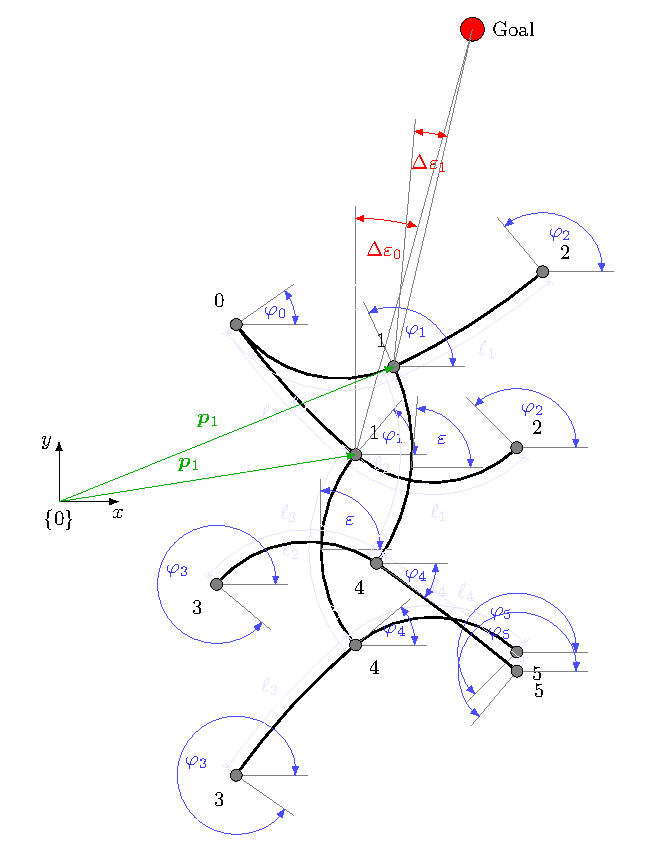
\includegraphics[width=8cm]{model.pdf}


\item Für die Pfadplanung, wäre eine Funktion hilfreich, die zu einer gegebenen Wunschdrehung $\Delta \varepsilon$, eine entsprechende Abfolge von Roboter-Konfigurationen / Posen ausgibt, sodass sich der Roboter entsprechend dreht.

\item So könnte zB die Richtung des Roboters so justiert werden, dass er sich auf ein gegebenes Ziel zu bewegt.


\item Für den geraden Gang ist eine analytische Funktion bekannt, die die Geschwindigkeit des Roboters einstellt. Geschwindigkeit im Sinne von Schrittweite, bzw. Vorschub pro Zyklus:

\begin{equation}
\bm{\alpha} = \begin{bmatrix}
45 - \frac{x_1}{2} \\
45 + \frac{x_1}{2} \\
x_1 \\
45 - \frac{x_1}{2}  \\
45 + \frac{x_1}{2} \\
\end{bmatrix}
\end{equation}

Die Schrittweite ist hier als $x_1$ beschrieben.

\end{itemize}




\section{Approach: Guess structure for a analytic model for walking curves}

\begin{itemize}

\item Src can be found: \texttt{analytic\_model.py}

\item Model:

\begin{equation}
\bm{\alpha} = \begin{bmatrix}
45 - \frac{x_1}{2} \\
45 + \frac{x_1}{2} \\
x_1 + x_2 \\
45 - \frac{x_1}{2}  \\
45 + \frac{x_1}{2} \\
\end{bmatrix}
\end{equation}

\item Method:

Simulate for different $x_1$ and $x_2$ (in der Abbildung unten ist $x_1$ = \texttt{gam} und $x_2$ = \texttt{x})

\item Results für 2 Zyklen:

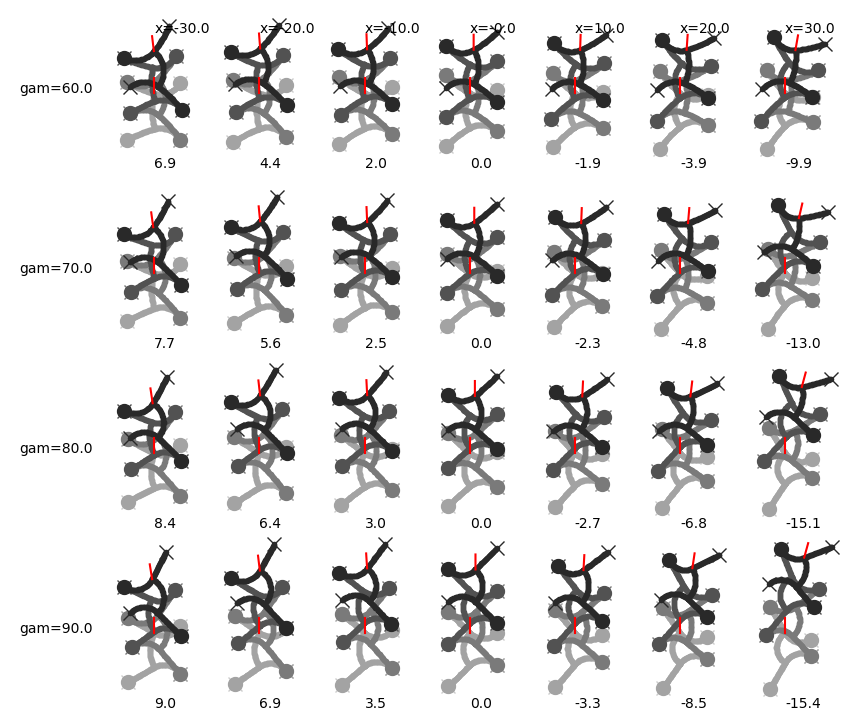
\includegraphics[width=12cm]{../pics/model_1/GeckoBotGait_2cyc.png}


\item Observations:

\begin{itemize}
	\item Es funktioniert. Der Roboter läuft eine Kurve.
	\item Kurve ist unsymmetrisch. Rechts klappt besser als links.
	\item Startpose ist besser für Rechtskurve geeignet.
	\item Noch nichts über die innere SPannung des Roboters herausgefunden
\end{itemize}



\end{itemize}


\section{Approach: Try another structure}

\begin{itemize}

\item Src can be found: \texttt{analytic\_model\_2.py}

\item Model:

\begin{equation}
\bm{\alpha} = \begin{bmatrix}
45 - \frac{x_1}{2} + \bar{f}_0|x_1x_2| + f_0|x1|x_2 \\
45 + \frac{x_1}{2} + \bar{f}_1|x_1x_2| + f_1|x1|x_2 \\
x_1 + |x_1|x_2 \\
45 - \frac{x_1}{2} + \bar{f}_2|x_1x_2| + f_2|x1|x_2 \\
45 + \frac{x_1}{2} + \bar{f}_3|x_1x_2| + f_3|x1|x_2 \\
\end{bmatrix}
\end{equation}


\item Results
\end{itemize}
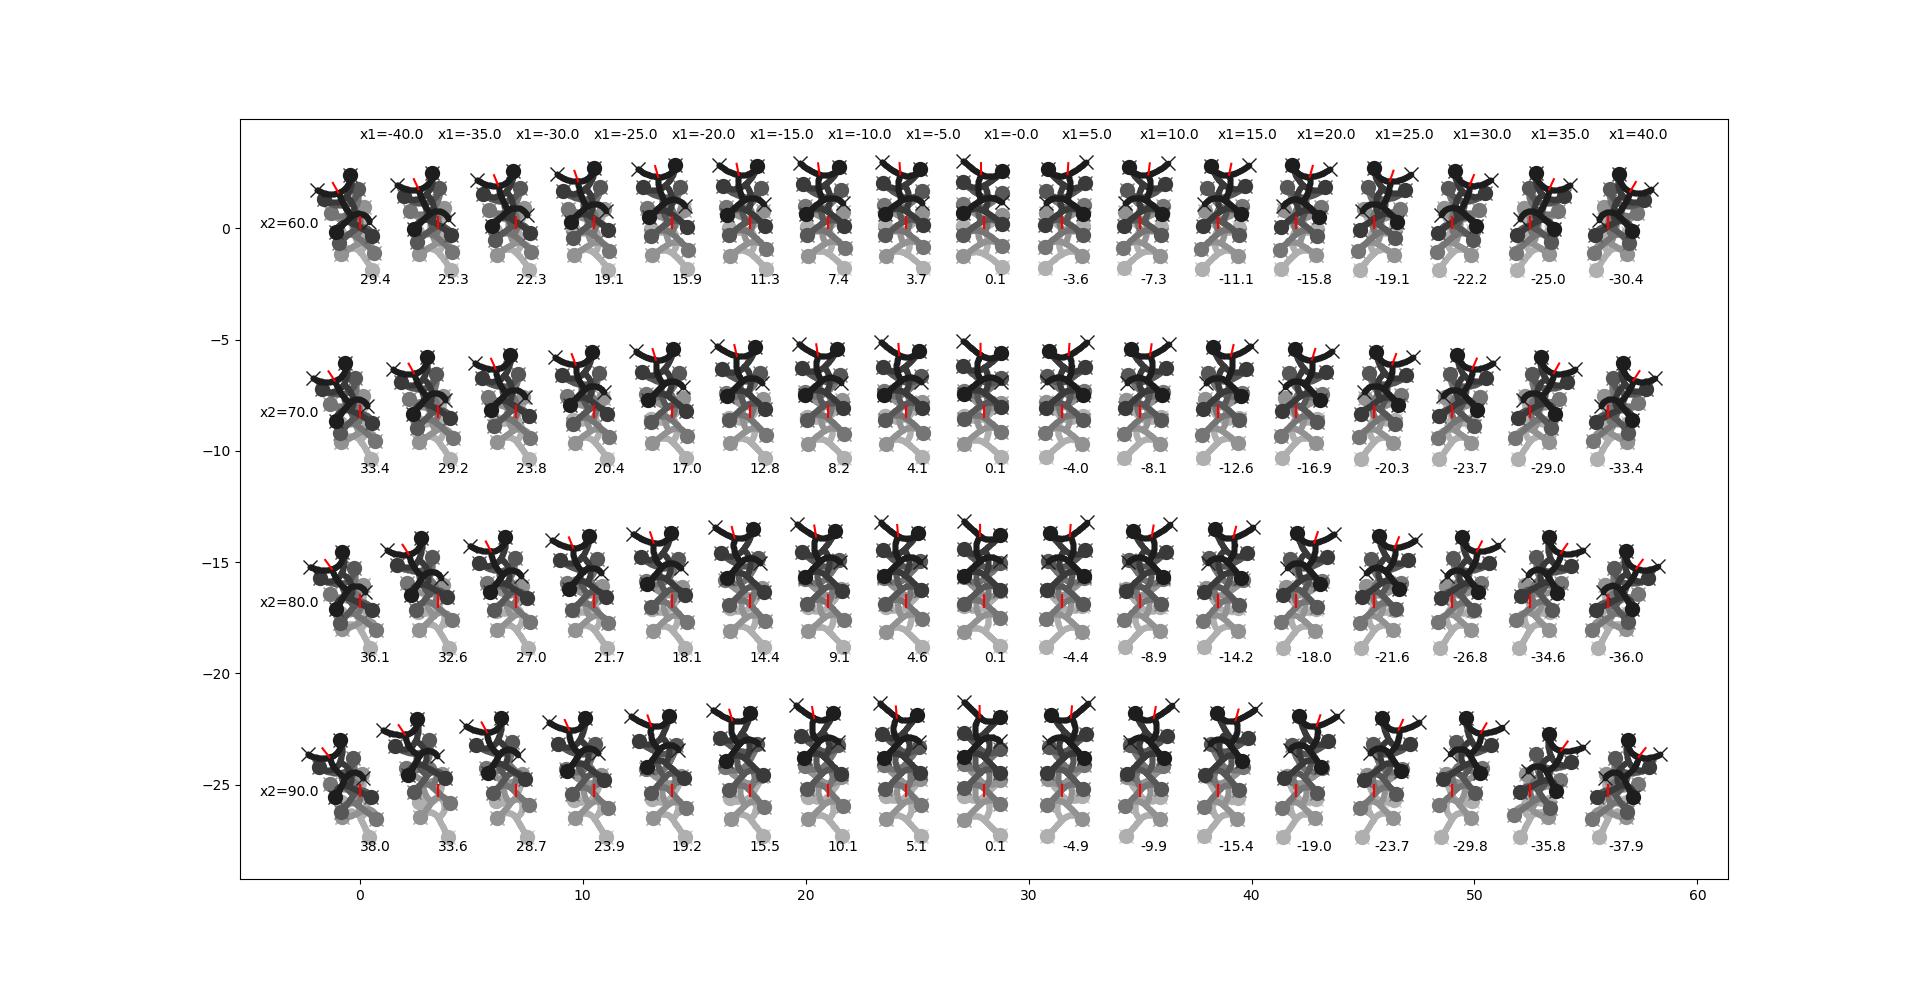
\includegraphics[width=.95\textwidth]{../pics/model_2/GeckoBotGait_003cyc_.png}

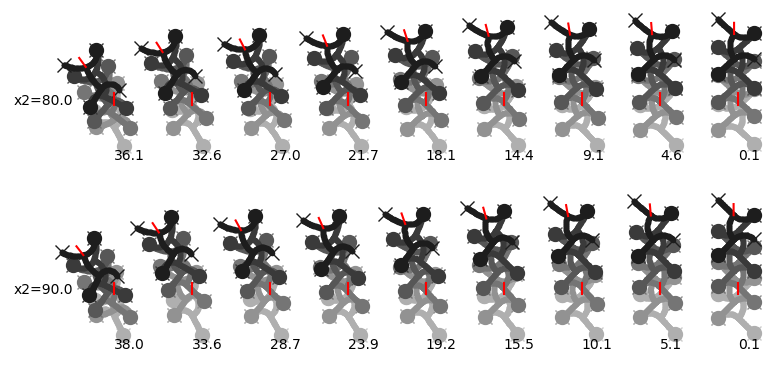
\includegraphics[width=.95\textwidth]{../pics/model_2/GeckoBotGait_003cyc_zoom.png}




\section{Approach: Optimize Extra leg bending Angle for given extra torso bending}

\begin{itemize}

\item Src can be found: \texttt{analytic\_model\_3.py}

\item Model:

\begin{equation}
\bm{\alpha} = \begin{bmatrix}
45 - \frac{x_1}{2} + \bar{f}_0x_3 + f_0x_4 \\
45 + \frac{x_1}{2} + \bar{f}_1x_3 + f_1x_4 \\
x_1 + x_2 \\
45 - \frac{x_1}{2} + \bar{f}_2x_4 + f_3x_3 \\
45 + \frac{x_1}{2} + \bar{f}_3x_4 + f_4x_3 \\
\end{bmatrix}
\end{equation}


\item Annahme:

Die Extra Biegung $x_3$ für freie Beine und die Extra Biegung $x_4$ für fixierte Beine sind abhängig von der Extra Biegung $x_2$ für den Torso.

\item Methode:

Für gegebenes Extra Torso Bending $x_2$ und gegebenene Torso Biegung $x1$ minimiere die Innere Spannung über den Gang mit $n$ Zyklen aufsummiert:

\begin{tabular}{c c l}
Gegeben: 	& $x_1$ & Torsobiegung \\
			& $x_2$	& Extra Torsobiegung \\
Gesucht:	& $x_3$	& Extra Beinbiegung fixiert vorn \\
			& $x_4$	& Extra Beinbiegung fixiert hinten \\

\end{tabular}


\begin{equation}
cost(\bm{x}) = \sum gait(\bm{x}).stress
\end{equation}

\item Observations:

Hinter- und Vorderbeine sind nicht symmetrisch, aber kreuzweise symmetrisch:
Die Extrabiegung für ein \textbf{nicht fixiertes Vorderbein} entspricht der Extrabiegung eines \textbf{fixierten Hinterbeins} und anderesherum.


\end{itemize}

\end{document}